% cd /disks/PROJECT/Mickael/COMMUNICATION/CST2016/;
% pdflatex Beamer_CST2016.tex; bibtex Beamer_CST2016; pdflatex Beamer_CST2016.tex; pdflatex Beamer_CST2016.tex
% evince Beamer_CST2016.pdf &

\documentclass[10pt, xcolors={RGB}, hyperref={pdfpagelabels=false,
        colorlinks=true,
        pdftex=true,
        bookmarks=true,
        bookmarksopen=true,
        hyperfootnotes=true}]{beamer}
\pdfpageattr{/Group << /S /Transparency /I true /CS /DeviceRGB>>}
\usepackage[T1]{fontenc}
\usepackage[utf8]{inputenc}
\usepackage{graphicx}
\usepackage{tabularx}
\usepackage{multirow}
\usepackage{pifont}
\usepackage{multicol}
\usepackage{setspace}
\renewcommand{\baselinestretch}{1.5}
\usepackage{helvet}
\renewcommand{\familydefault}{\sfdefault}
\usepackage[square, authoryear]{natbib}

\definecolor{dodgerblue}{RGB}{30,144,255}
\definecolor{springgreen3}{RGB}{0,139,69}
\definecolor{springgreen2}{RGB}{0,205,102}
\definecolor{firebrick2}{RGB}{238,44,44}
\definecolor{maroon2}{RGB}{238,48,167}
\definecolor{goldenrod2}{RGB}{238,180,34}
\definecolor{deepskyblue}{RGB}{0,191,255}



\usetheme{CambridgeUS}
\useoutertheme{infolines}
\useinnertheme{rectangles}
\setbeamercolor{frametitle}{fg=white, bg=springgreen3!90!black!60!white}
\setbeamercolor{title}{fg=white, bg=springgreen3!50!white}
\setbeamercolor{palette primary}{fg=springgreen3!40!black, bg=springgreen3!50!white}
\setbeamercolor{palette secondary}{fg=springgreen3!30!black, bg=springgreen3!70!white}
\setbeamercolor{palette tertiary}{fg=springgreen3!20!black, bg=springgreen3!90!white}
\setbeamercolor{structure}{fg=springgreen3!70!white}
\setbeamercolor{background canvas}{bg=white}
\setbeamercolor{normal text}{fg=black}
\setbeamercolor{block title}{bg=dodgerblue, fg=white!75!dodgerblue}
\setbeamercolor{example text}{fg=springgreen3}
\setbeamercolor{block title example}{bg=springgreen3, fg=white!75!springgreen3}
\setbeamercolor{alerted text}{fg=firebrick2}
\setbeamercolor{block title alerted}{bg=firebrick2, fg=white!75!firebrick2}
\setbeamertemplate{navigation symbols}{}
\addtobeamertemplate{headline}{\hypersetup{allcolors=springgreen3!40!black}}{}

\def\cst#1{\def\@cst{#1}}
\defbeamertemplate*{title page}{custom}[1][]{
    \renewcommand{\baselinestretch}{1.25}
    \begin{centering}
        \begin{beamercolorbox}[sep=3pt,center,#1]{institute}
            \usebeamerfont{institute}{\insertinstitute}
        \end{beamercolorbox}
        \vfill
        \begin{beamercolorbox}[sep=8pt, center, colsep=-4bp, rounded=true, shadow=true, #1]{title}
            \usebeamerfont{title}\inserttitle\par%
            \ifx\insertsubtitle\@empty%
            \else%
            \vskip0.25em%
            {\usebeamerfont{subtitle}\usebeamercolor[fg]{subtitle}\insertsubtitle\par}%
            \fi%
        \end{beamercolorbox}%
        \vskip1em\par
        \begin{beamercolorbox}[sep=8pt,center,#1]{author}
            \usebeamerfont{author}\insertauthor
        \end{beamercolorbox}
        \begin{beamercolorbox}[sep=8pt,center,#1]{cst}
            \usebeamerfont{institute}\@cst
        \end{beamercolorbox}
        \begin{beamercolorbox}[sep=8pt,center,#1]{date}
            \usebeamerfont{date}{\small\insertdate}
        \end{beamercolorbox}
        \vfill
        {\usebeamercolor[fg]{titlegraphic}\inserttitlegraphic\par}
    \end{centering}
    \renewcommand{\baselinestretch}{1.5}
}



\hypersetup{%
    linkcolor=dodgerblue,
    urlcolor=firebrick2,
    citecolor=springgreen3,
    filecolor=goldenrod2,
    menucolor=dodgerblue,
    bookmarksopen=true}
\renewcommand{\thefootnote}{\textcolor{maroon2}{\arabic{footnote}}}

\usepackage{textcomp}
\usepackage{listings}
\usepackage{courier}

\newcommand\bref[2]{\hyperref[#1]{#2~\ref*{#1}}}
\newcommand\cmd[1]{\texttt{\color{black}\textbf{#1}}}
\newcommand\cmdb[1]{\texttt{\color{dodgerblue}\textbf{#1}}}
\newcommand\cmdr[1]{\texttt{\color{firebrick2}\textbf{#1}}}
\newcommand\cmdg[1]{\texttt{\color{springgreen3}\textbf{#1}}}
\newcommand\cmdy[1]{\texttt{\color{goldenrod2}\textbf{#1}}}
\newcommand\blue[1]{{\color{dodgerblue}\textbf{#1}}}
\newcommand\red[1]{{\color{firebrick2}\textbf{#1}}}
\newcommand\green[1]{{\color{springgreen3}\textbf{#1}}}
\newcommand\yellow[1]{{\color{goldenrod2}\textbf{#1}}}
\newcommand\pql{{\rmfamily \textbf{\color{goldenrod2}``}}}
\newcommand\pqr{{\rmfamily \textbf{\color{goldenrod2}''}}}
\newcommand\pq[3]{{\rmfamily \textbf{\color{#3}``}}#1{\rmfamily \textbf{\color{#3}''}} - \textcolor{#3}{#2}}
\newenvironment{bquote}[1]
    {\begin{quotation}
    \vspace{10pt}
    \newcommand{\bqauthor}{\normalfont \begin{quote}\begin{flushright}--- #1\end{flushright}\end{quote}}
    \rmfamily \itshape {\huge\textbf{``}}
    }
    {{\huge\textbf{''}}
    \bqauthor
    \end{quotation}
    }

\usepackage[english, francais]{babel}
% \usepackage[english]{babel}
\selectlanguage{francais}

% \AtBeginSection[]
% {
  % \begin{frame}
    % \frametitle{Sommaire}
    % \tableofcontents[sectionstyle=show/hide, subsectionstyle=show/hide/hide]
  % \end{frame}
% }




\date[26 Septembre 2016]{%
    {\color{springgreen3!70!white}26 Septembre 2016}
}

\author[Mickaël Canouil]{%
    \texorpdfstring{Mickaël Canouil\\ \vskip -0.25cm
    \href{mailto:mickael.canouil@cnrs.fr}{{\scriptsize mickael.canouil@cnrs.fr}}}{Mickaël Canouil}
}

\institute[CNRS UMR 8199]{%
    {\color{springgreen3!90!white}\blue{G}énomique \blue{I}ntégrative et \blue{M}odélisation des \blue{M}aladies \blue{M}étaboliques
    \linebreak UMR 8199 (CNRS / Université de Lille 2 / Institut Pasteur de Lille)}%
}

\titlegraphic{%
    
\includegraphics[height=1cm, keepaspectratio]{../UTILS/Logos/logo_cnrs.pdf}\hspace{1.5cm}
    
\includegraphics[height=1cm, keepaspectratio]{../UTILS/Logos/UL2-WEB-2014.png}\hspace{1.5cm}
    
\includegraphics[height=1cm, keepaspectratio]{../UTILS/Logos/Institut-Pasteur-de-Lille.png}\hspace{1.5cm}
    
\includegraphics[height=1cm, keepaspectratio]{../UTILS/Logos/logo_egid.pdf}%
}

\title[\texorpdfstring{\color{black}CST 2016}{}]{%
    Développement et Application de Méthodologies Statistiques pour Etudes Longitudinales d'Association Génétique%
}

\subtitle{%
    \textit{Comité de suivi de thèse: deuxième année}
}

\cst{{\color{springgreen3!90!white}\textbf{Direction de thèse}}\\ Dr. Ghislain Rocheleau \& Pr. Philippe Froguel}


\graphicspath{{figures/}}


\usepackage{tikz}
\usebackgroundtemplate{%
    \shorthandoff{;}%
    \tikz\node[opacity=0.20, inner sep=0pt] {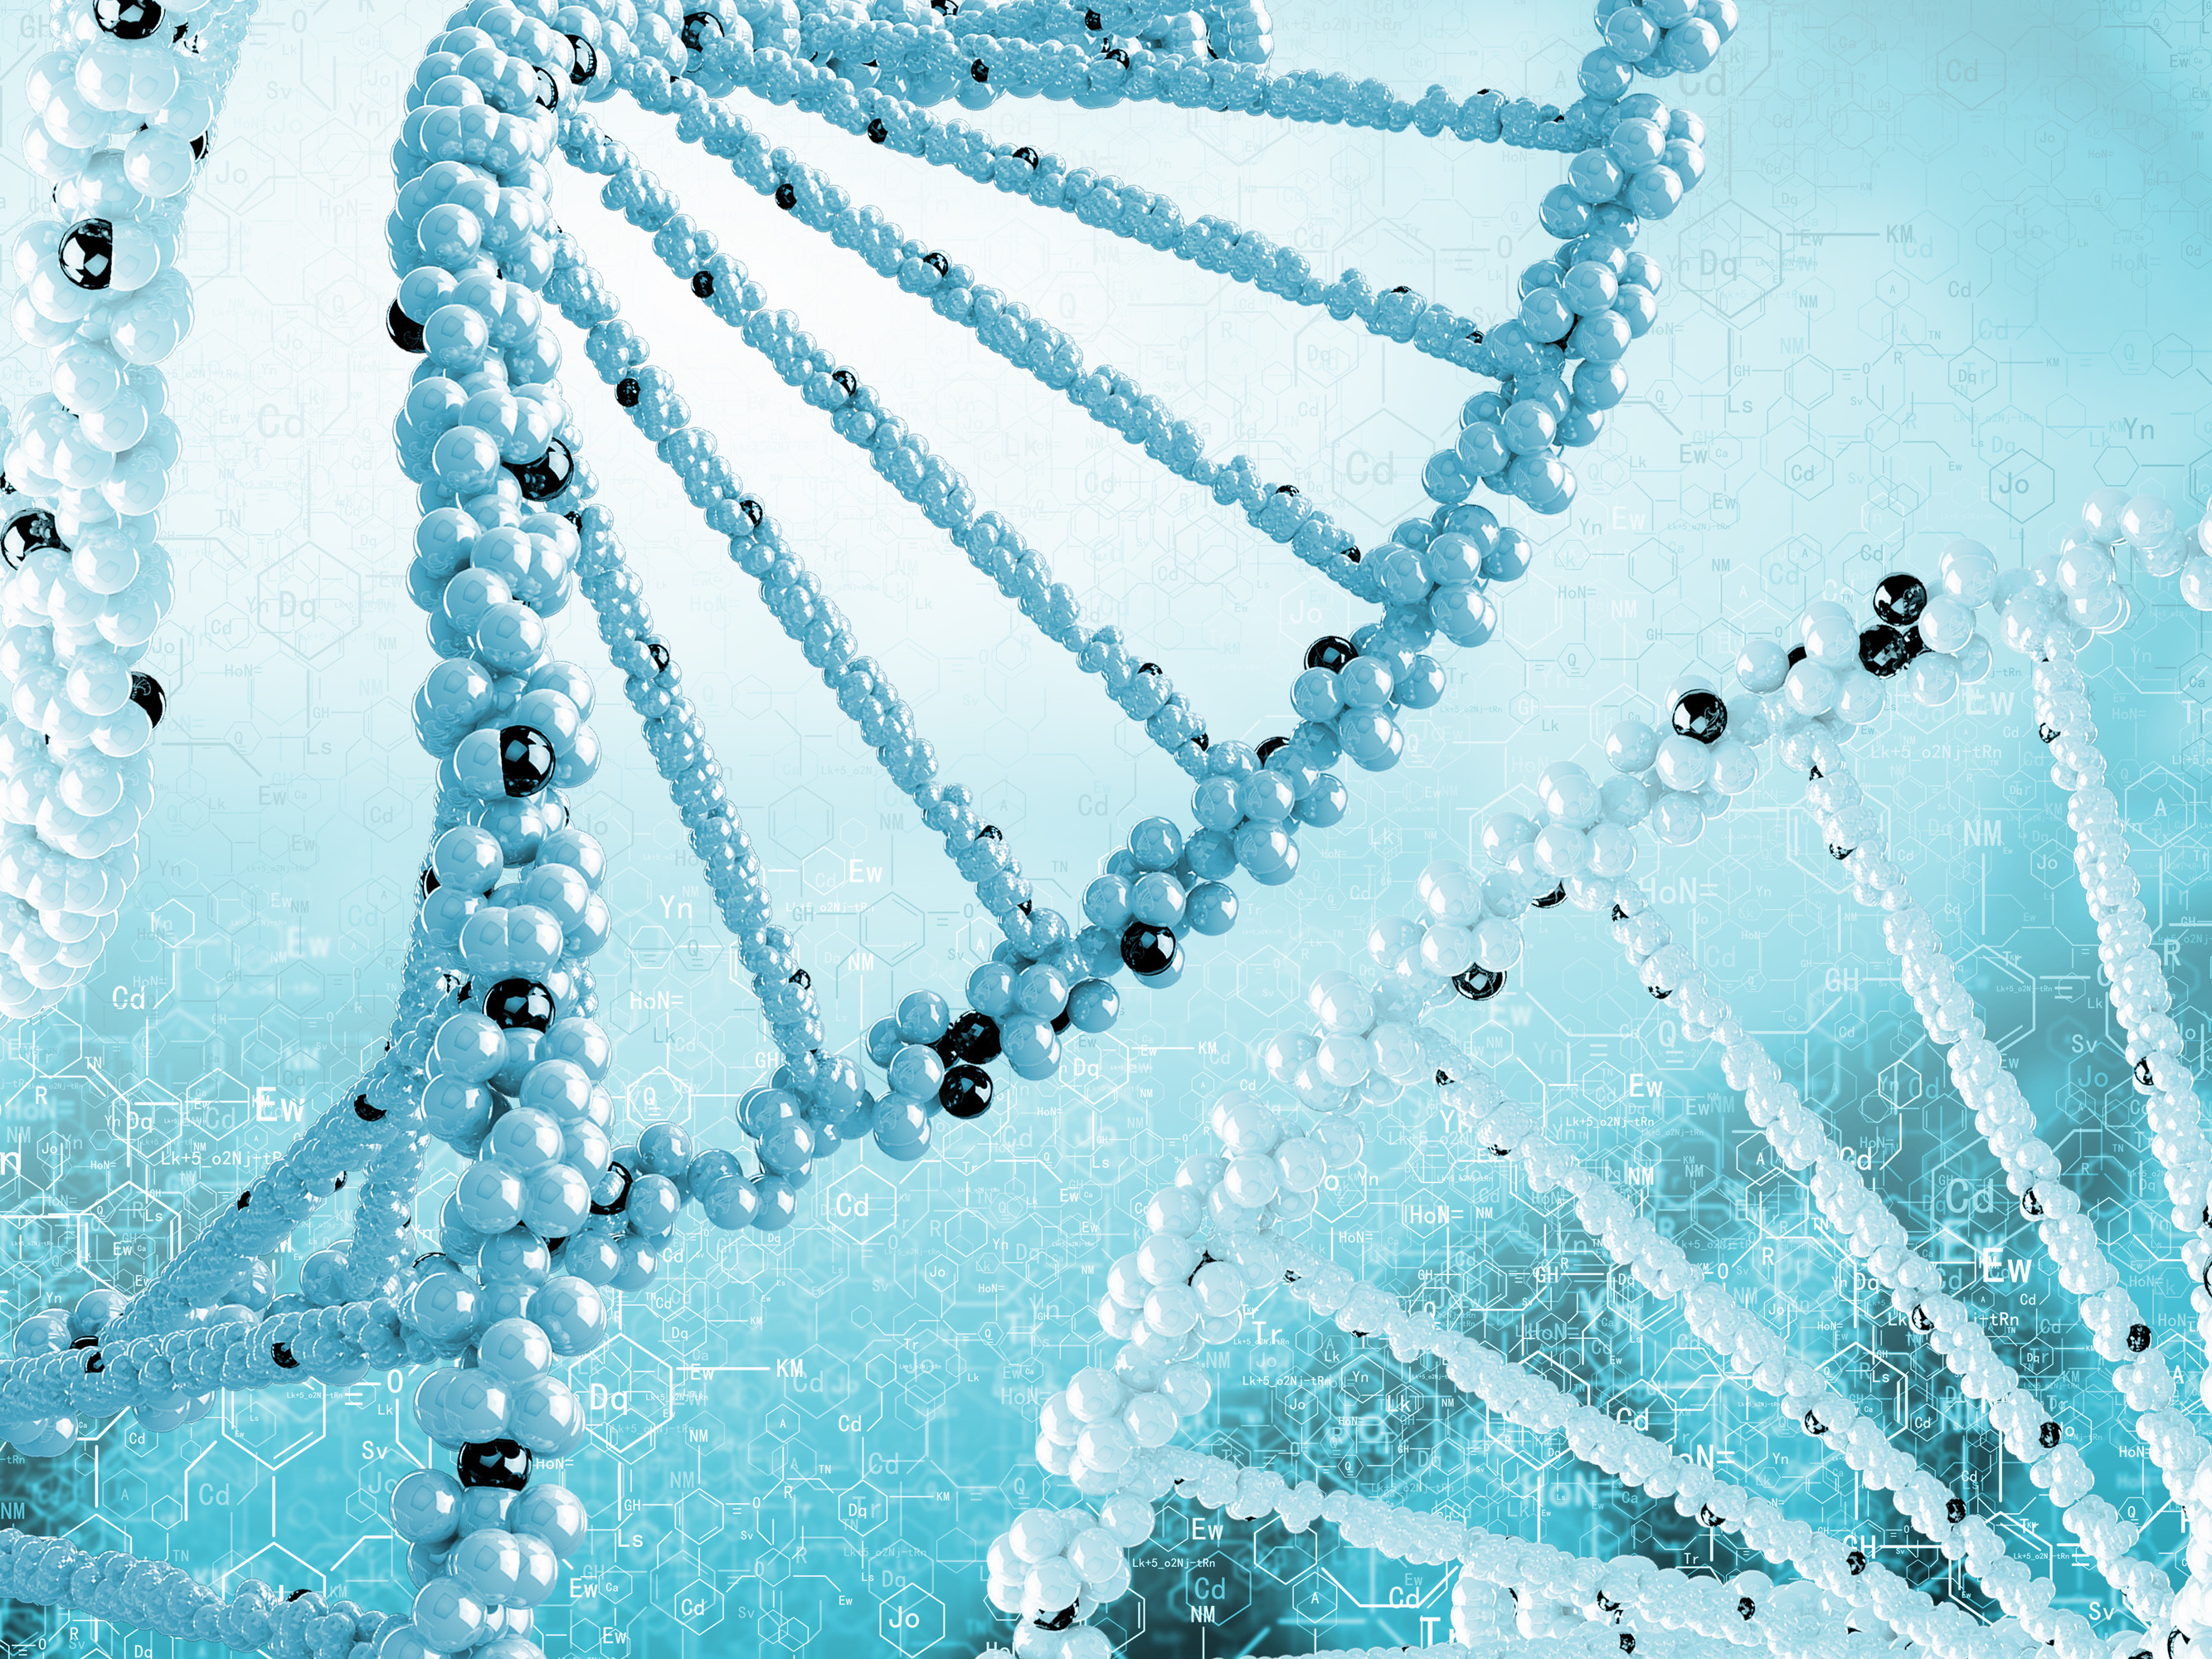
\includegraphics[height=\paperheight, width=\paperwidth]{../UTILS/Background/BG03_Beamer.jpg}};%
}


\begin{document}
\maketitle
\begin{frame}{{\huge\textcolor{dodgerblue}{$\mathcal{S}$}}ommaire}
    \vspace{-3em}
    \begin{multicols}{2}
        \noindent
        \tableofcontents[sectionstyle=show/show, subsectionstyle=hide/hide/hide, subsubsectionstyle=hide/hide/hide, sections={1-4}]
        \columnbreak
        \tableofcontents[sectionstyle=show/show, subsectionstyle=hide/hide/hide, subsubsectionstyle=hide/hide/hide, sections={5-8}]
    \end{multicols}
\end{frame}


\section{Introduction}
\begin{frame}{{\huge\textcolor{dodgerblue}{$\mathcal{I}$}}ntroduction}
\par{En \textcolor{springgreen3}{2014}, la prévalence de diabète de type 2 (\textcolor{springgreen3}{DT2}) a été estimée à près de
\textcolor{springgreen3}{9\%} chez l'adulte de \textcolor{springgreen3}{18} ans et plus.}
\vspace{1em}
\par{Sur la dernière décennie, l'essor des études d'association pangénomiques (\textcolor{springgreen3}{GWAS}) a permis l'identification de:
    \begin{itemize}
        \item \textcolor{springgreen3}{65} variants associés à la susceptibilité au \textcolor{springgreen3}{DT2};
        \item \textcolor{springgreen3}{36} variants associés à la glycémie à jeun (\textcolor{springgreen3}{FG}) chez les normoglycémiques.
    \end{itemize}
}
\end{frame}


\begin{frame}{{\huge\textcolor{dodgerblue}{$\mathcal{I}$}}ntroduction}
\par{La grande majorité des \textcolor{springgreen3}{GWAS} a utilisé un design transversal, quand un design longitudinal offre la possibilité:
    \begin{itemize}
        \item de décrire la trajectoire temporelle d'une variable;
        \item d'accroître la puissance pour détecter des variants génétiques associés à la trajectoire.
    \end{itemize}
}
\vspace{1em}
\par{La modélisation de ces trajectoires temporelles optimiserait les tests d'association et l'exploitation des phenotypes disponibles.}
\end{frame}


\section{Objectifs}
\begin{frame}{{\huge\textcolor{dodgerblue}{$\mathcal{O}$}}bjectifs}
\par{Cette thèse s'organise sur deux principaux objectifs:
\begin{enumerate}
    \item Développement et implémentation des approches basées notamment sur les modèles joints;
    \item Application à un jeu de données (p.ex. cohorte \textcolor{springgreen3}{D.E.S.I.R.}, \textcolor{springgreen3}{FRAMINGHAM}, etc);
    \vspace{1em}
    \item Optimisation du temps de calcul avec \textcolor{springgreen3}{R} (p.ex. \textcolor{springgreen3}{lme4}, portage \textcolor{springgreen3}{Julia}, etc).
\end{enumerate}
}
\end{frame}

\section{Matériels}
\begin{frame}{{\huge\textcolor{dodgerblue}{$\mathcal{M}$}}atériels}{}
{\small
\par{Le laboratoire (\textcolor{springgreen3}{UMR CNRS 8199}) dispose de l'accès à la cohorte prospective \textcolor{springgreen3}{D.E.S.I.R.}
(\textcolor{springgreen3}{D}onnées \textcolor{springgreen3}{E}pidémiologiques sur le \textcolor{springgreen3}{S}yndrome d’\textcolor{springgreen3}{I}nsulino-\textcolor{springgreen3}{R}ésistance),
comptant \textcolor{springgreen3}{5~212} individus suivis pendant \textcolor{springgreen3}{9} ans, tous les
\textcolor{springgreen3}{3 ans} (\textcolor{springgreen3}{0}, \textcolor{springgreen3}{3}, \textcolor{springgreen3}{6}
et \textcolor{springgreen3}{9} ans).}
\vspace{1em}
\par{En plus de données phénotypiques (p.ex. \textcolor{springgreen3}{FG}, \textcolor{springgreen3}{hba1c}, etc), des données génotypiques sont également disponibles
pour une grande partie de ces individus (\textcolor{springgreen3}{4~364}): \\ \textcolor{springgreen3}{124~095 SNPs} (fréquence allèlique \textcolor{springgreen3}{$>1\%$} et Hardy-Weinberg \textcolor{springgreen3}{$p<1 \times 10^{-3}$}).}
\vspace{1em}
\par{Cette cohorte comporte \textcolor{springgreen3}{179} cas incidents de \textcolor{springgreen3}{DT2}, définis à partir
d'une glycémie supérieure à \textcolor{springgreen3}{7 mmol/L} ou par la prise d'un traitement anti-diabétique.}
}
\end{frame}


\section{Méthodes}
\subsection{Modèle Joint}
\begin{frame}{{\huge\textcolor{dodgerblue}{$\mathcal{M}$}}éthodes: Modèle Joint}
\par{L'approche par modèle joint a éré décrite par \textcolor{dodgerblue}{\cite{tsiatis2004}} et \textcolor{dodgerblue}{\cite{ibrahim_basic_2010}},\\
avec une implémentation  dans l'extension \textcolor{springgreen3}{JM} \textcolor{dodgerblue}{\citep{rizopoulos_jm_2010}} du logiciel \textcolor{springgreen3}{R} (version 3.2.3)\textcolor{dodgerblue}{\citep{r_core_team_r_2015}}.}

\begin{minipage}[t]{0.475\columnwidth}
    \vspace{0.2cm}
    \begin{center}
        \fbox{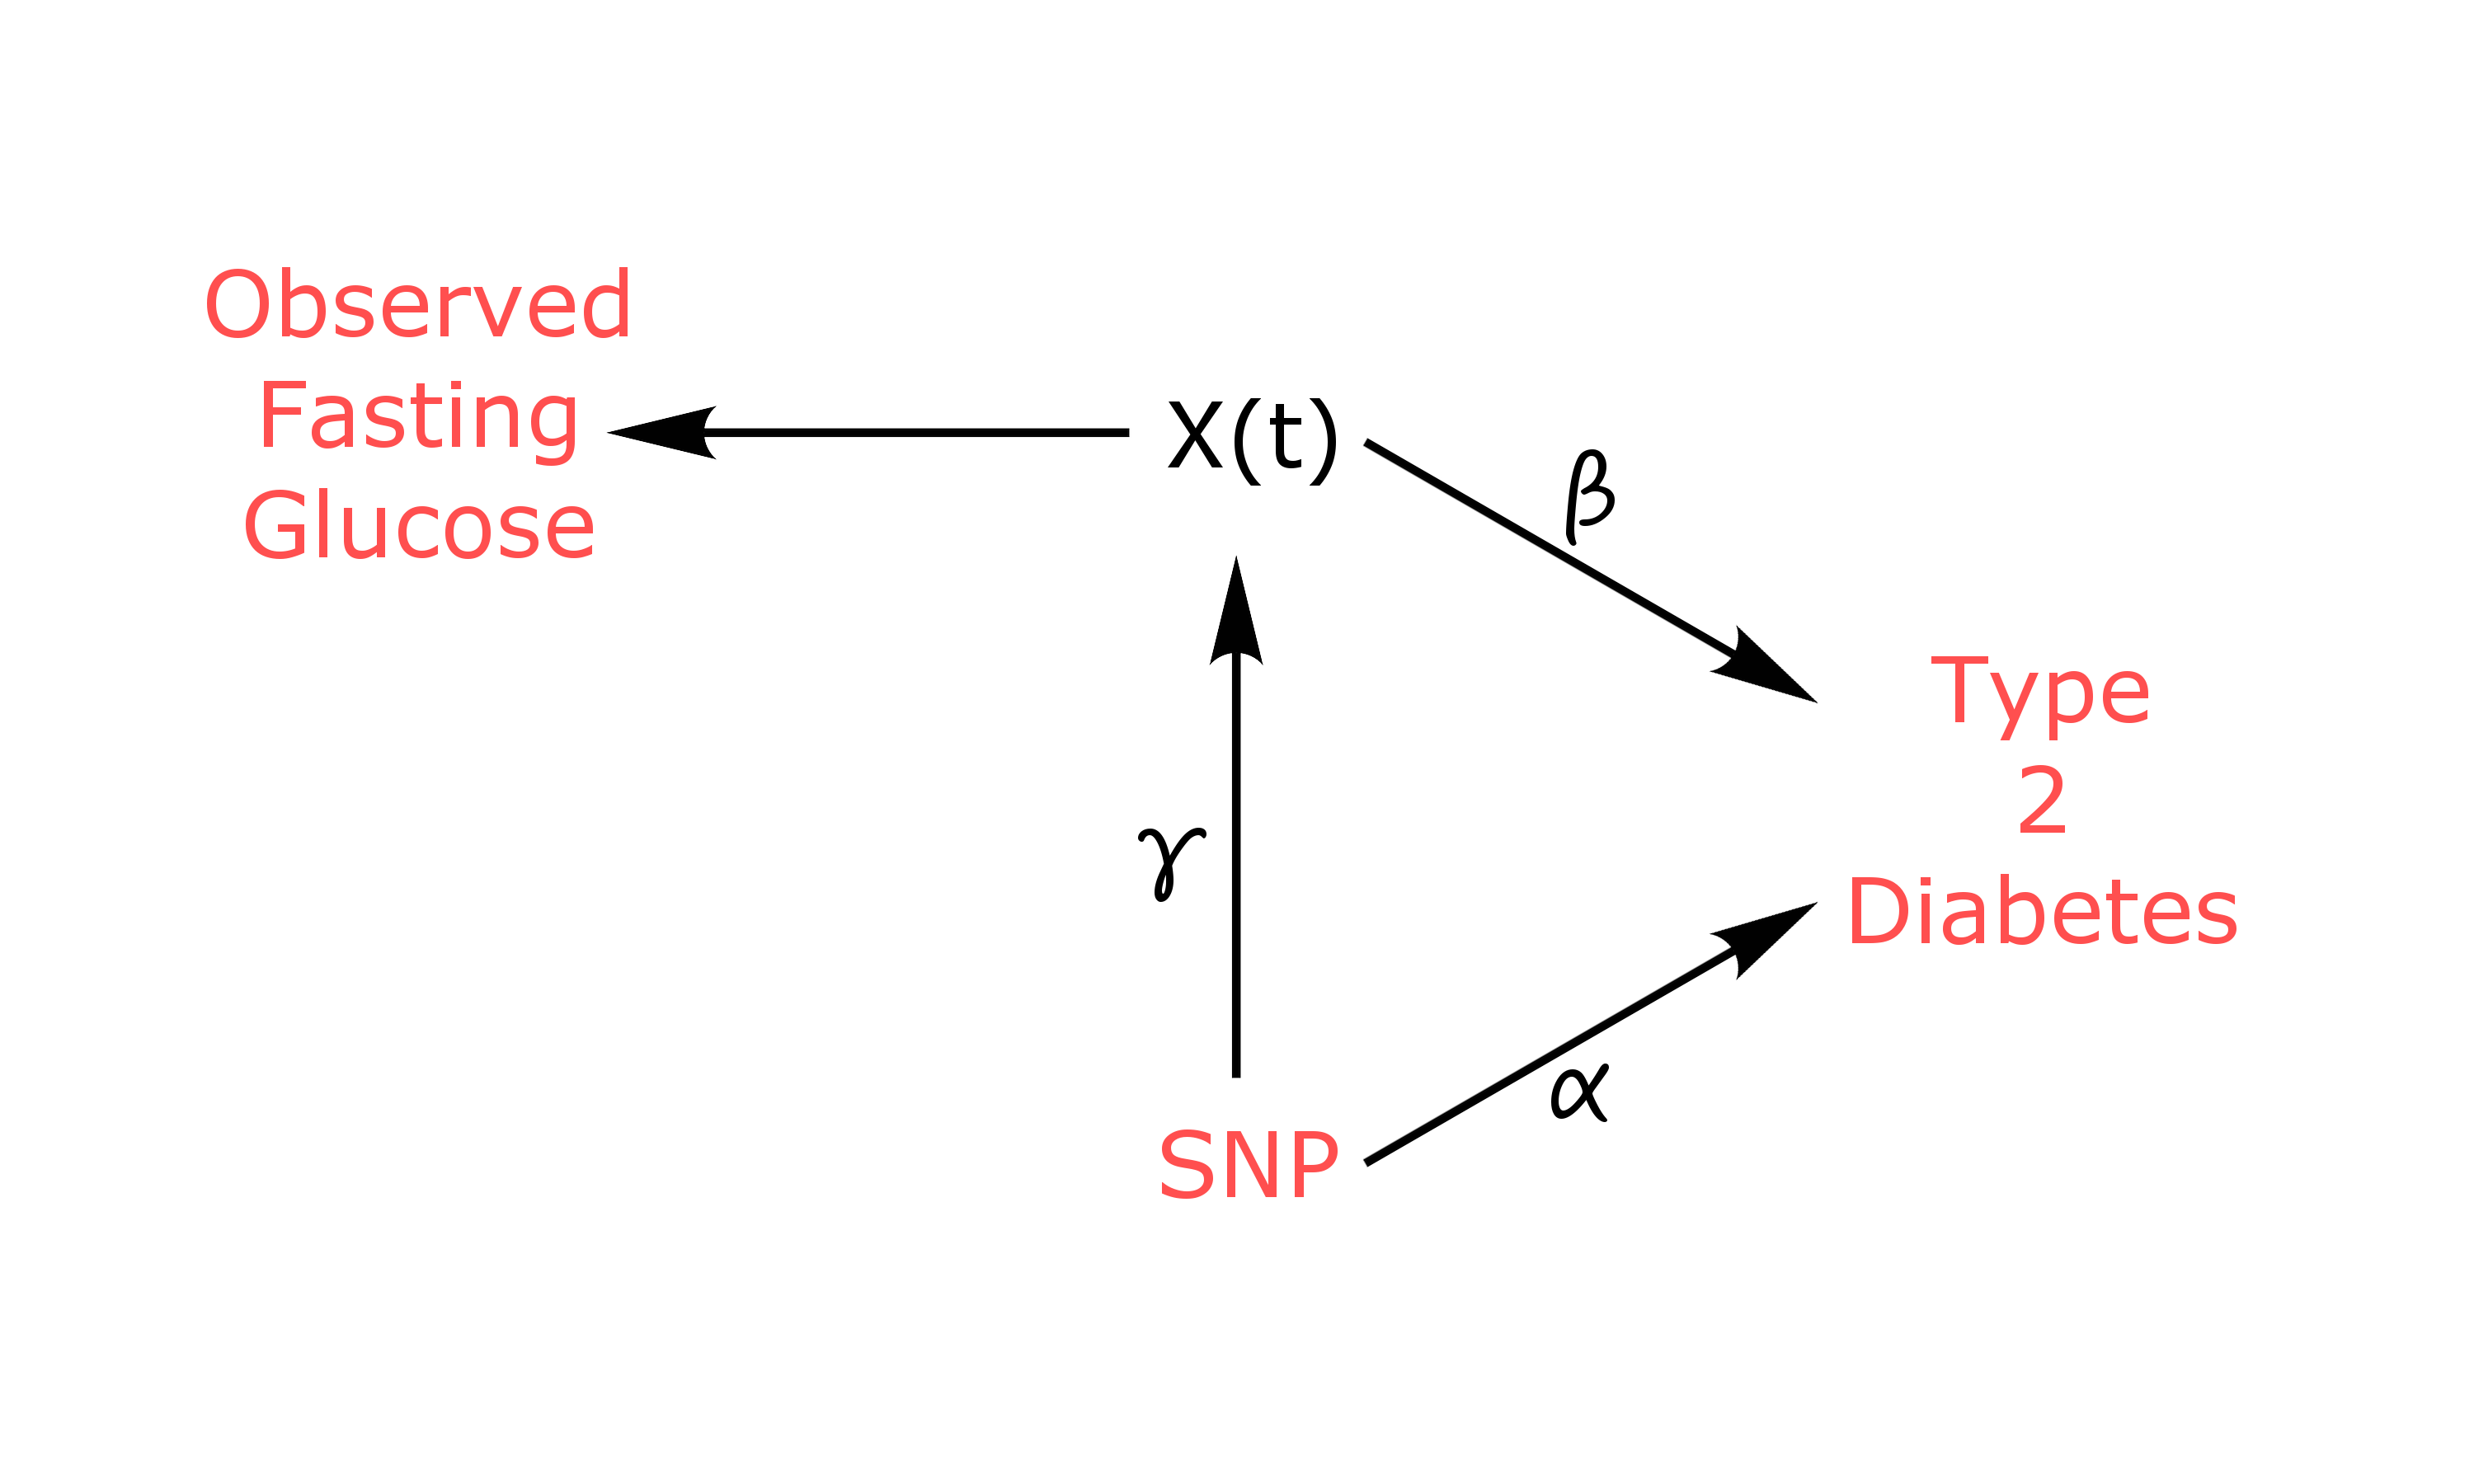
\includegraphics[width=5cm]{figures/jointModel.png}}
    \end{center}
\end{minipage}%
\hfill\vline\hfill
\begin{minipage}[t]{0.475\columnwidth}%
    % \vspace{-2cm}
    \par{\footnotesize \textcolor{springgreen3}{$X(t)$}: trajectoire de \textcolor{springgreen3}{FG} inférée des données longitudinales observées;\\
    \textcolor{springgreen3}{$\alpha$}: effet du SNP sur le \textcolor{springgreen3}{DT2};\\
    \textcolor{springgreen3}{$\gamma$}: effet du SNP sur la trajectoire de \textcolor{springgreen3}{FG};\\
    \textcolor{springgreen3}{$\beta$}: effet de la trajectoire de \textcolor{springgreen3}{FG} sur le \textcolor{springgreen3}{DT2}.}
\end{minipage}
\end{frame}

\begin{frame}{{\huge\textcolor{dodgerblue}{$\mathcal{M}$}}éthodes: Modèle Joint}
\par{Le modèle joint se décompose en deux parties:
\begin{itemize}
    \item Composante longitudinale (Modèle linéaire mixte)
        \textcolor{springgreen3}{
            \begin{eqnarray}Y_{ij}=X_{ij}+\epsilon_{ij}\label{eq:1}\end{eqnarray}
            \begin{eqnarray}Y_{ij}=\theta_{0i}+\theta_{1i}\times t_{ij} + \gamma \times Z_i + (\delta \times W_i) + \epsilon_{ij}\label{eq:2}\end{eqnarray}
            \begin{eqnarray}\boldsymbol\theta \sim \mathcal{N}_2(\boldsymbol\mu, \boldsymbol\Sigma)\nonumber\label{Eq3};\quad \epsilon_{ij} \sim \mathcal{N}(0, \sigma^2)\nonumber\label{Eq4}\end{eqnarray}
        }
    \item Composante de survie (Modèle de Cox)
        \textcolor{springgreen3}{\begin{eqnarray}h_i(t)=h_0(t) exp(\beta X_i(t)+\alpha Z_i)\label{eq:3}\end{eqnarray}}
\end{itemize}
}
\end{frame}


\subsection{Simulation}
% \subsubsection{Modèle}
\begin{frame}{{\huge\textcolor{dodgerblue}{$\mathcal{M}$}}éthodes: Simulation}%{Modèle}
\par{Simulation des données selon les \hyperref[eq:1]{Equations~\ref*{eq:1}~à~\ref{eq:3}}, avec la fonction de risque de base fixée: \textcolor{springgreen3}{$h_0(t)=\lambda$}.}
\par{Les temps d'événements ont été générés selon une distribution exponentielle (Cox à risque proportionnel) \textcolor{dodgerblue}{\citep{austin_generating_2012}}.
\textcolor{springgreen3}{\begin{eqnarray}H(T)=\int_0^T \lambda exp(\beta \times X(t) + \alpha \times Z) dt\end{eqnarray}}
\textcolor{springgreen3}{\begin{eqnarray}T=\frac{1}{\beta\theta_1} log\left( - \frac{\beta\theta_1 \times log(1-u)}{\lambda exp(\beta\theta_0+(\beta\gamma+\alpha)Z)}+1 \right)\end{eqnarray}}
}
\end{frame}

% \subsubsection{Etude du modèle joint}
\begin{frame}{{\huge\textcolor{dodgerblue}{$\mathcal{M}$}}éthodes: Simulation}%{Etude du modèle joint}
\par{Paramètres initiaux pour la simulation des données basés sur le SNP de \textcolor{springgreen3}{TCF7L2} (SNP le plus fortement associé au \textcolor{springgreen3}{DT2}).}
{\footnotesize \begin{center}
    \begin{tabular}{lc}
        \hline
        Paramètres & Valeurs\\
        \hline
        Effectif ($N$) & $5000$\\
        Temps de mesures (en années) & $0, 3, 6, 9$\\
        Incidence à neuf ans ($I$) & $5\%$\\
        LMM : Trajectoire $\left (\begin{bmatrix}\theta_{0}\\\theta_{1}\end{bmatrix}\right )$ & $\mathcal{N}_2\left (\begin{bmatrix}4.50\\0.013\end{bmatrix} , \begin{bmatrix} 0.16 & 0 \\ 0 & 1\times 10^{-3} \end{bmatrix} \right )$\\
        LMM : Effet du SNP ($\gamma$) & $0.025$\\
        Cox : Effet du SNP ($\alpha$) & $0.2$\\
        JM : Effet de la trajectoire ($\beta$) & $3.50$\\
        \hline
    \end{tabular}
\end{center}}
\end{frame}


\section{Résultats}
\subsection{Simulation}
\begin{frame}{{\huge\textcolor{dodgerblue}{$\mathcal{S}$}}imulation}{$\alpha$: effet du SNP sur le diabète}
    {\small \begin{center}
        \begin{tabular}{ccccc}
            \hline
            Paramètre & Estimée & Simulée & Fréquence allélique\\
            \hline
            \multirow{7}{*}{$\alpha$} & \textcolor{maroon2}{0.215 [-0.0762, 0.551]} & \multirow{7}{*}{0.23} & 0.05 \\
             & 0.219 [0.00346, 0.459] &  & 0.10 \\
             & 0.22 [0.0741, 0.373] &  & 0.25 \\
             & 0.219 [0.101, 0.343] &  & 0.50 \\
             & 0.219 [0.0825, 0.349] &  & 0.75 \\
             & 0.218 [0.0284, 0.398] &  & 0.90 \\
             & \textcolor{maroon2}{0.218 [-0.0538, 0.461]} &  & 0.95 \\
            \hline
        \end{tabular}
    \end{center}}
\end{frame}
\begin{frame}{{\huge\textcolor{dodgerblue}{$\mathcal{S}$}}imulation}{$\beta$: effet du SNP sur la trajectoire de la glycémie à jeun}
    {\small \begin{center}
        \begin{tabular}{ccccc}
            \hline
            Paramètre & Estimée & Simulée & Fréquence allélique\\
            \hline
            \multirow{7}{*}{$\beta$} & 3.56 [3.29, 3.85] & \multirow{7}{*}{3.60} & 0.05 \\
             & 3.57 [3.3, 3.85] &  & 0.10 \\
             & 3.57 [3.3, 3.86] &  & 0.25 \\
             & 3.56 [3.29, 3.85] &  & 0.50 \\
             & 3.57 [3.29, 3.85] &  & 0.75 \\
             & 3.57 [3.29, 3.85] &  & 0.90 \\
             & 3.57 [3.29, 3.85] &  & 0.95 \\
            \hline
        \end{tabular}
    \end{center}}
\end{frame}
\begin{frame}{{\huge\textcolor{dodgerblue}{$\mathcal{S}$}}imulation}{$\gamma$: effet de la trajectoire de la glycémie à jeun sur le diabète}
    {\small \begin{center}
        \begin{tabular}{ccccc}
            \hline
            Paramètre & Estimée & Simulée & Fréquence allélique\\
            \hline
            \multirow{7}{*}{$\gamma$} & \textcolor{maroon2}{0.0196 [-0.0164, 0.0558]} & \multirow{7}{*}{0.02} & 0.05 \\
             & \textcolor{maroon2}{0.0195 [-0.00712, 0.0456]} &  & 0.10 \\
             & 0.0194 [0.00111, 0.038] &  & 0.25 \\
             & 0.0197 [0.00322, 0.0353] &  & 0.50 \\
             & 0.0196 [0.00115, 0.0385] &  & 0.75 \\
             & \textcolor{maroon2}{0.0196 [-0.00678, 0.0457]} &  & 0.90 \\
             & \textcolor{maroon2}{0.0195 [-0.0165, 0.0558]} &  & 0.95 \\
            \hline
        \end{tabular}
    \end{center}}
\end{frame}

\begin{frame}{{\huge\textcolor{dodgerblue}{$\mathcal{S}$}}imulation}
\par{\`A partir des résultats de simulations, nous pouvons recommandés les conditions suivantes (pour une incidence de 5\%):
\vspace{1em}
\begin{itemize}
    \item Fréquence allélique $>5\%$
    \vspace{0.5em}
    \item Nombre de mesures $>4$
    \vspace{0.5em}
    \item Taille de population $\>1~000$
    \vspace{0.5em}
    \item Données manquantes (MCAR/MAR) $<25\%$
\end{itemize}
}
\end{frame}


\subsection{Application D.E.S.I.R.}
\begin{frame}{{\huge\textcolor{dodgerblue}{$\mathcal{H}$}}istorique}{}
\par{Identification de 80 et 100 loci associés au DT2 et au FG, notamment via GWAS et méta-analyses \textcolor{dodgerblue}{\citep{dupuis_new_2010, yaghootkar_recent_2013, vaxillaire_type_2014}}.}
\begin{center}
    \fbox{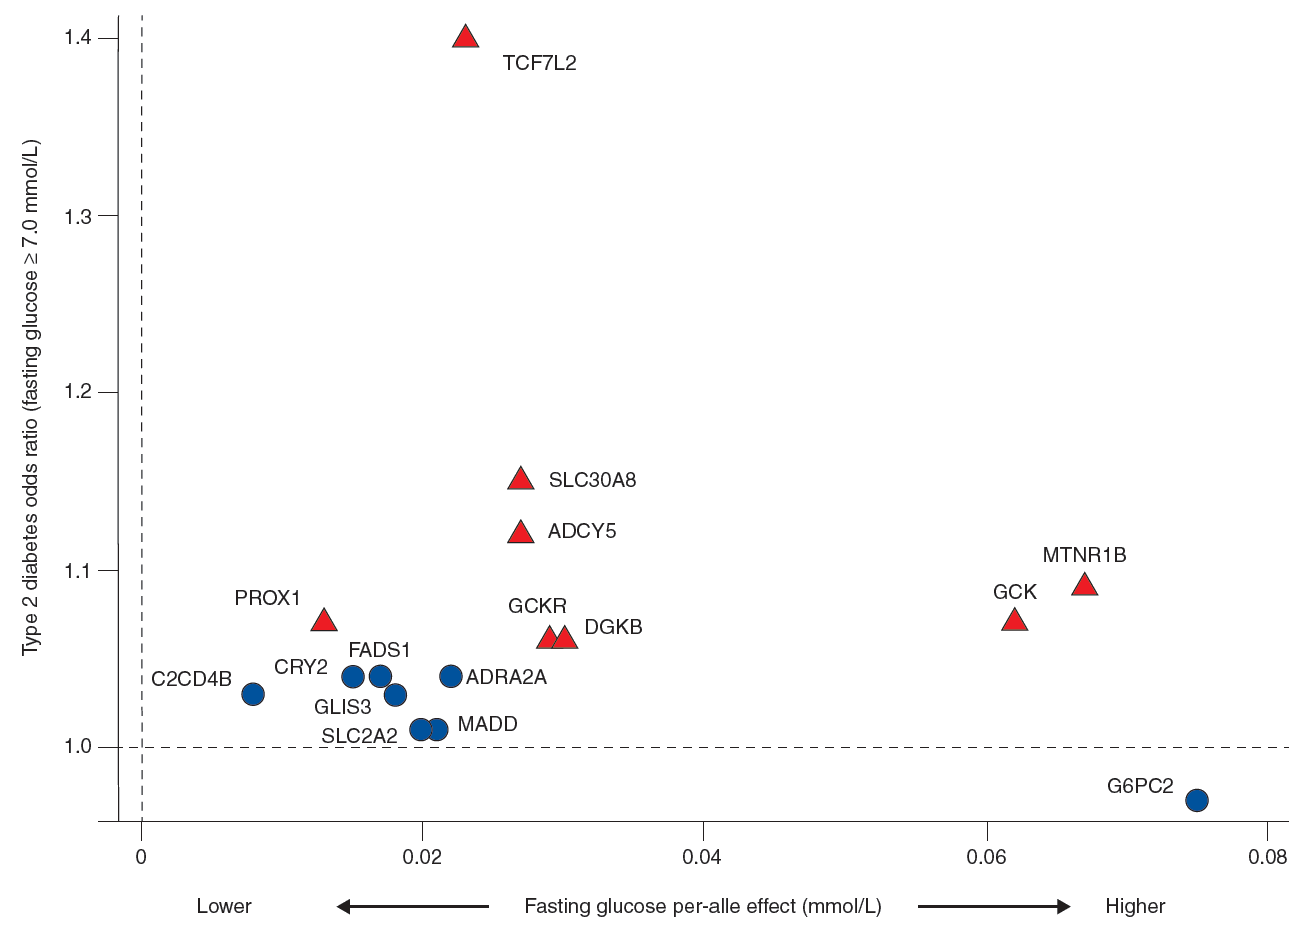
\includegraphics[width=7cm]{figures/Yaghootkar.png}}
\end{center}
\end{frame}

\begin{frame}{{\huge\textcolor{dodgerblue}{$\mathcal{A}$}}pplication D.E.S.I.R.}{}
\begin{center}
    \fbox{\includegraphics[width=8cm]{/disks/DATA/DESIR_longitudinal/16-JointModel_MetaboChipSimu/JAV2016_Figure2.png}}
\end{center}
\vspace{-1em}
{\footnotesize
\begin{minipage}[t]{0.475\columnwidth}
\par{\begin{itemize}
\item 124~095 SNPs ont été analysés dans la cohorte \textcolor{springgreen3}{D.E.S.I.R.} avec la puce MetaboChip \textcolor{dodgerblue}{\citep{voight_metabochip_2012}}.
\end{itemize}}
\end{minipage}%
\hfill\vline\hfill
\begin{minipage}[t]{0.475\columnwidth}%
\par{\begin{itemize}
\item \textcolor{springgreen3}{145} loci trouvés comme associés à la fois à \textcolor{springgreen3}{FG} et à la survenue du \textcolor{springgreen3}{DT2} (au seuil de \textcolor{springgreen3}{5\%})
\end{itemize}}
\end{minipage}
}
\end{frame}

\begin{frame}{{\huge\textcolor{dodgerblue}{$\mathcal{A}$}}pplication D.E.S.I.R.}{}
\par{La puissance statistique a été calculée:
\vspace{1em}
\begin{enumerate}
    \item au niveau du modèle joint, à l'aide de la formule de \textcolor{dodgerblue}{\citet{chen_sample_2011}}:
{\scriptsize \textcolor{springgreen3}{\begin{eqnarray}z_{\tilde{\beta}}=&\pm\sqrt{Df(1-f)(\beta\gamma+\alpha)^2}+z_{1-\tilde{\alpha}/2}\nonumber\end{eqnarray}}}
avec\vspace{-1em}
\begin{description}
    \item[\textcolor{springgreen3}{$D$}] le nombre de \textcolor{springgreen3}{DT2} incidents,
    \item[\textcolor{springgreen3}{$f$}] la fréquence de l'allèle à risque,
\end{description}
\vspace{1em}
    \item au niveau des paramètres \textcolor{springgreen3}{$\gamma$} et \textcolor{springgreen3}{$\alpha$} respectivement pour l'effet du SNP sur la trajectoire de \textcolor{springgreen3}{FG} et sur le risque de \textcolor{springgreen3}{DT2}.
\end{enumerate}
}
\end{frame}


\begin{frame}{{\huge\textcolor{dodgerblue}{$\mathcal{A}$}}pplication D.E.S.I.R.}{}
\begin{center}
    \input{"/disks/DATA/DESIR_longitudinal/16-JointModel_MetaboChipSimu/JAV2016_Table1.tex"}
    \par{\scriptsize (En \textcolor{dodgerblue}{bleu}: $\textrm{p-value}<0.05$, en \textcolor{firebrick2}{rouge}: $\textrm{p-value}<5\times 10^{-8}$)}
\end{center}
\end{frame}

\begin{frame}{{\huge\textcolor{dodgerblue}{$\mathcal{A}$}}pplication D.E.S.I.R.}{}
\par{En \textcolor{dodgerblue}{bleu}, lorsque le modèle joint (\textcolor{springgreen3}{JM}) présente une puissance statistique supérieure à une approche transversale (CM): régression linéaire/logistique (\textcolor{springgreen3}{JM} / \textcolor{springgreen3}{CM}).}
\begin{center}
    \input{"/disks/DATA/DESIR_longitudinal/16-JointModel_MetaboChipSimu/JAV2016_Table2.tex"}
    \par{\scriptsize (Erreur de type 1: $5.81\%\pm0.83$ / $5.47\%\pm0.64$ pour \textcolor{springgreen3}{JM} et \textcolor{springgreen3}{CM})}
\end{center}
\end{frame}


\section{Performance}
\begin{frame}{{\huge\textcolor{dodgerblue}{$\mathcal{P}$}}erformance}{}
\begin{center}
    \fbox{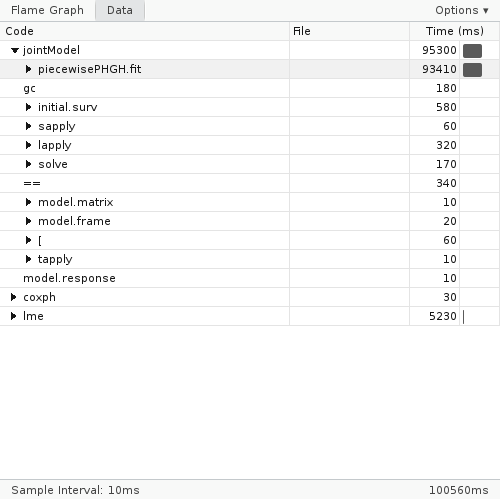
\includegraphics[width=5cm]{./figures/Perf0.png}}
    \fbox{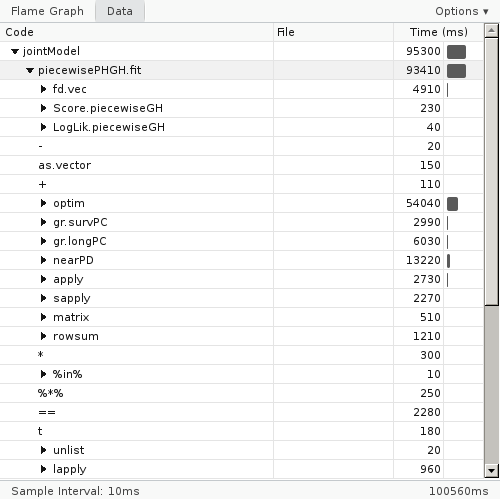
\includegraphics[width=5cm]{./figures/Perf1.png}}
\end{center}
\end{frame}
\begin{frame}{{\huge\textcolor{dodgerblue}{$\mathcal{P}$}}erformance}{}
\par{Malgré les optimisations apportées au niveau des paramètres de convergence de l'étape EM du modèle joint (extension \textcolor{springgreen3}{JM} \textcolor{dodgerblue}{\citep{rizopoulos_jm_2010}}),
qui représente \textcolor{springgreen3}{50\%} du temps total,
il est possible d'apporter d'autres optimisations de façon simple: comme l'utilisation des fonctions de bas niveau de \textcolor{springgreen3}{R}:}
\begin{center}
    \fbox{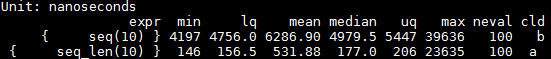
\includegraphics[width=8cm]{./figures/exOptim.png}}
\end{center}
\end{frame}

\section{Perspectives}
\begin{frame}{{\huge\textcolor{dodgerblue}{$\mathcal{P}$}}erspectives}
\par{%
\begin{enumerate}
    \item Ecriture d’un \textcolor{springgreen3}{rapport scientifique} (Bourse SFD-Lilly: 21 Mai 2017) et d'un \textcolor{springgreen3}{article sur l'application du modèle joint à la cohorte D.E.S.I.R.}
    \item \textcolor{springgreen3}{Validation des SNPs/gènes} mis en évidence par le modèle joint (p.ex. cohorte de réplication)
    \item Etude d'autre trait tel que l'\textcolor{springgreen3}{HbA1c} (hémoglobine glyquée)
    \item Inclusion des individus incident pour l'\textcolor{springgreen3}{IFG} (Impaired Fasting Glucose; $FG>6.1mM/L$) en plus des individus DT2 ($FG>7mM/L$)
    \item \textcolor{springgreen3}{Optimisation} du code (algorithme de JM) pour une exécution sur des puces GWAS et/ou imputées
\end{enumerate}
}
\end{frame}


\section{Congrès}
\begin{frame}{{\huge\textcolor{dodgerblue}{$\mathcal{C}$}}ongrès}
\begin{itemize}
    \item \textcolor{springgreen3}{\textit{SMPGD 2016}} (Statistical Methods for Post Genomic Data): \\Présentation orale \\{\footnotesize "Longitudinal Genetic Modelling: Revisiting Associations of SNPs Associated with Blood Fasting Glucose in Normoglycemic Individuals"}
    \vspace{1em}
    \item \textcolor{springgreen3}{\textit{IGES 2016}} (International Genetic Epidemiology Society): \\Présentation poster \\{\footnotesize "Single Nucleotide Polymorphisms Associated With Fasting Blood Glucose Trajectory And Type 2 Diabetes Incidence: A Joint Modelling Approach"}
\end{itemize}
\end{frame}

\begin{frame}{{\huge\textcolor{dodgerblue}{$\mathcal{C}$}}ongrès}
\begin{itemize}
    \item \textcolor{springgreen3}{\textit{SFD 2017}} (Société Francophone du Diabète)
    \item \textcolor{springgreen3}{\textit{SFdS 2017}} (Société Française de Statistique)
    \item \textcolor{springgreen3}{\textit{Rencontres R 2017}}
    \item \textcolor{springgreen3}{\textit{useR 2017}}
\end{itemize}
\end{frame}


\section{Références}
\begin{frame}<beamer:0>{{\huge\textcolor{dodgerblue}{$\mathcal{R}$}}éférences}
    \bibliographystyle{apalike}
    \bibliography{CST2016.bib}
\end{frame}


\end{document}